\documentclass{article}
\usepackage{amsmath}
\usepackage{graphicx} 
\usepackage{booktabs}

\title{Assignment 4: Stock Market Prediction using Recurrent Neural
Networks}
\author{Logan Nunno }
\date{April 2026}

\begin{document}

\maketitle

\section{Introduction}

In this assignment, we investigate the use of recurrent neural networks (RNNs) for stock market prediction. Unlike traditional feedforward neural networks, recurrent models are designed to handle sequential data, making them well-suited for time series forecasting such as stock prices.

We evaluate three models:
\begin{itemize}
    \item Basic RNN (baseline)
    \item Gated Recurrent Unit (GRU)
    \item Long Short-Term Memory (LSTM)
\end{itemize}

We use historical stock data from four companies: AAPL, GOOG, AMD, and NVDA. The goal is to predict the next day's closing price based on the previous 50 days.

\section{Task 2}

The initial phase of the project involved establishing a baseline using a standard Recurrent Neural Network. Unlike traditional feedforward networks, RNNs process sequences by maintaining a hidden state $h_t$ that acts as a memory of previous inputs. The state update is governed by the following recurrence:
\begin{equation}
    h_t = \sigma(W_{hh}h_{t-1} + W_{xh}x_t + b_h)
\end{equation}

For this implementation, I utilized a sliding window of $M=50$ days to predict the closing price of the following day ($N=1$). To ensure stable training, the raw price data was normalized using a \texttt{MinMaxScaler} to a $[0, 1]$ range based on the training split (80\% of the data).


The baseline model is a multi-layer RNN implemented using PyTorch. The architecture consists of:
\begin{itemize}
    \item Input size: 1 (closing price)
    \item Hidden size: 64
    \item Stacked Layers: A 2-layer RNN was used to allow the model to learn hierarchical features.
    \item Dropout: A dropout rate of 0.2 was applied to mitigate overfitting, forcing the network to learn robust feature representations.
    \item Batch Normalization: Applied to the final hidden state output to stabilize gradients before the fully connected prediction layer.
\end{itemize}

The model takes a sequence of 50 previous stock prices and predicts the next value. The hidden state from the final time step is passed through batch normalization and then into a linear layer.

The intuition behind this structure is that the RNN captures temporal dependencies in stock prices, while batch normalization helps stabilize training and improve convergence.

The results for the Basic RNN were strong, as shown in Table 1.
\begin{table}[h]
    \centering
    \caption{Basic RNN Performance Metrics}
    \begin{tabular}{lccccc}
        \toprule
        Ticker & MAE & MSE & RMSE & MAPE (\%) & Accuracy (\%) \\
        \midrule
        AAPL & 6.0501 & 53.2660 & 7.2984 & 2.55\% & 97.45\% \\
        GOOG & 5.4066 & 70.4841 & 8.3955 & 2.28\% & 97.72\% \\
        AMD  & 5.3240 & 53.0930 & 7.2865 & 3.38\% & 96.62\% \\
        NVDA & 4.8018 & 38.0187 & 6.1659 & 3.48\% & 96.52\% \\
        \bottomrule
    \end{tabular}
\end{table}

Training time was approximately 7.8 seconds per stock.

\subsection{Prediction Visualization}

\begin{figure}[h]
\centering
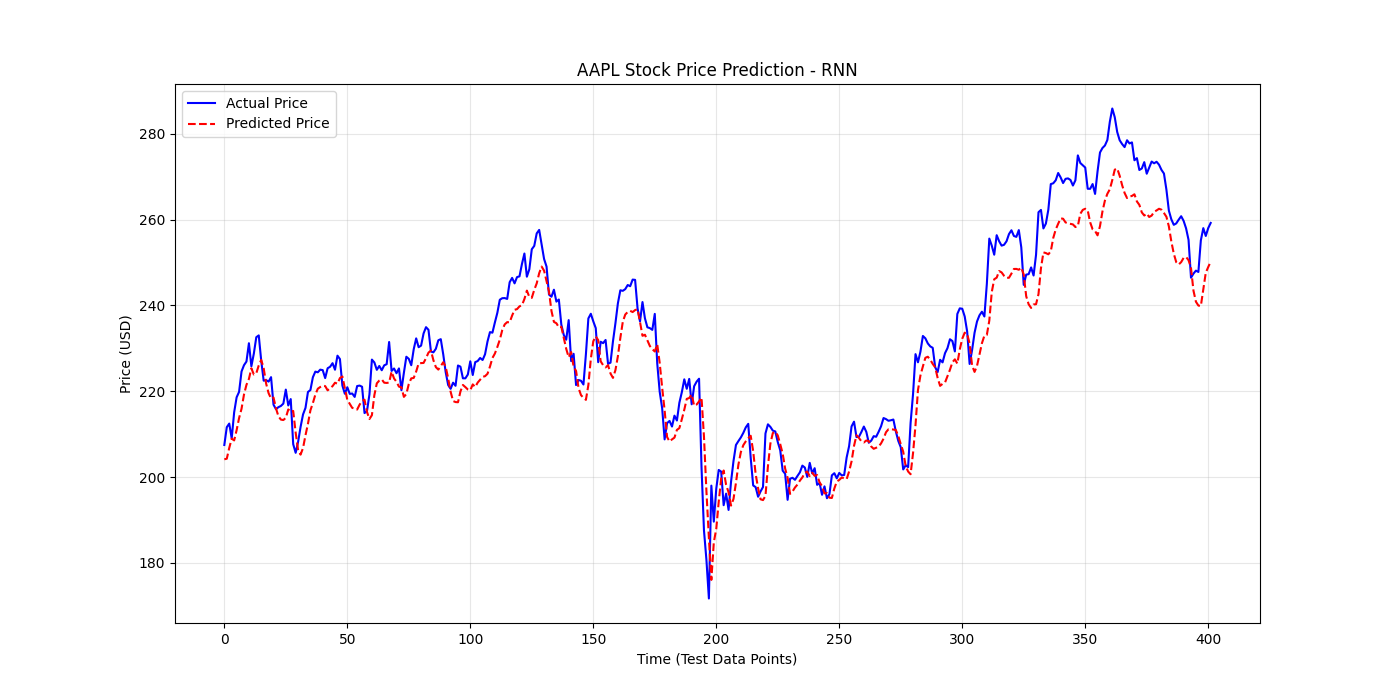
\includegraphics[width=0.8\textwidth]{stock_plots/AAPL_RNN_prediction.png}
\caption{AAPL Prediction vs Actual (RNN)}
\end{figure}

\section{Task 3}

\section{Task 4}

\section{Task 5}


\end{document}